\section{Анализ предметной области}
\label{sec:analysis}

Извлечение музыкальной информации - небольшая, но интересная и быстрорастущая область исследований, которая охватывает большой диапазон продуктов, используемых по всему миру. Эта область охватывает \\несколько дисциплин научных знаний: музыковедение, психологию, обработку сигналов, машинное обучение и комбинации этих дисциплин. Задача, которую будет решать разрабатываемый сервис, относится к задачам извлечения музыкальной информации.

Несмотря на то, что извлечение музыкальной информации является еще небольшой областью исследований, для извлечения характеристик музыкальных приложений применяется достаточное количество методов. Эти методы различаются как на основаниии применяемых подходов, так и на основании уровней извлекаемых характеристик. На основании характеристик выделяют методы, которые извлекают низкоуровневые характеристики (спектр, ритм), и методы которые извлекают высокоуровневые характеристики (жанр, настроение). В основном, нас будут интересовать методы, которые извлекают высокоуровневые характеристики.

Для извлечения высокоуровневых характеристик выделяют два класса методов: основанные на математических функциях, в основе которых лежит машинное обучение. В музыке появляются новые направления, а старые могут изменяться, поэтому наиболее перспективными являются методы, которые способны постраиваться под переменчивую природу музыки. Под такие условия в большей степени подходят методы, в основе которых лежит машинное обучение.

Машинное обучение - класс методов, характерной чертой которых является не прямое решение задачи, а решение, которое строится в процессе обучения при применении решения к множеству сходных задач. В последнее время этот класс методов получил активное развитие и поддержку со стороны крупных компаний и университетов.

Цифровой аудиосигнал можно представить в виде изображения звуковой волны.

\begin{figure}[t]
\centering
	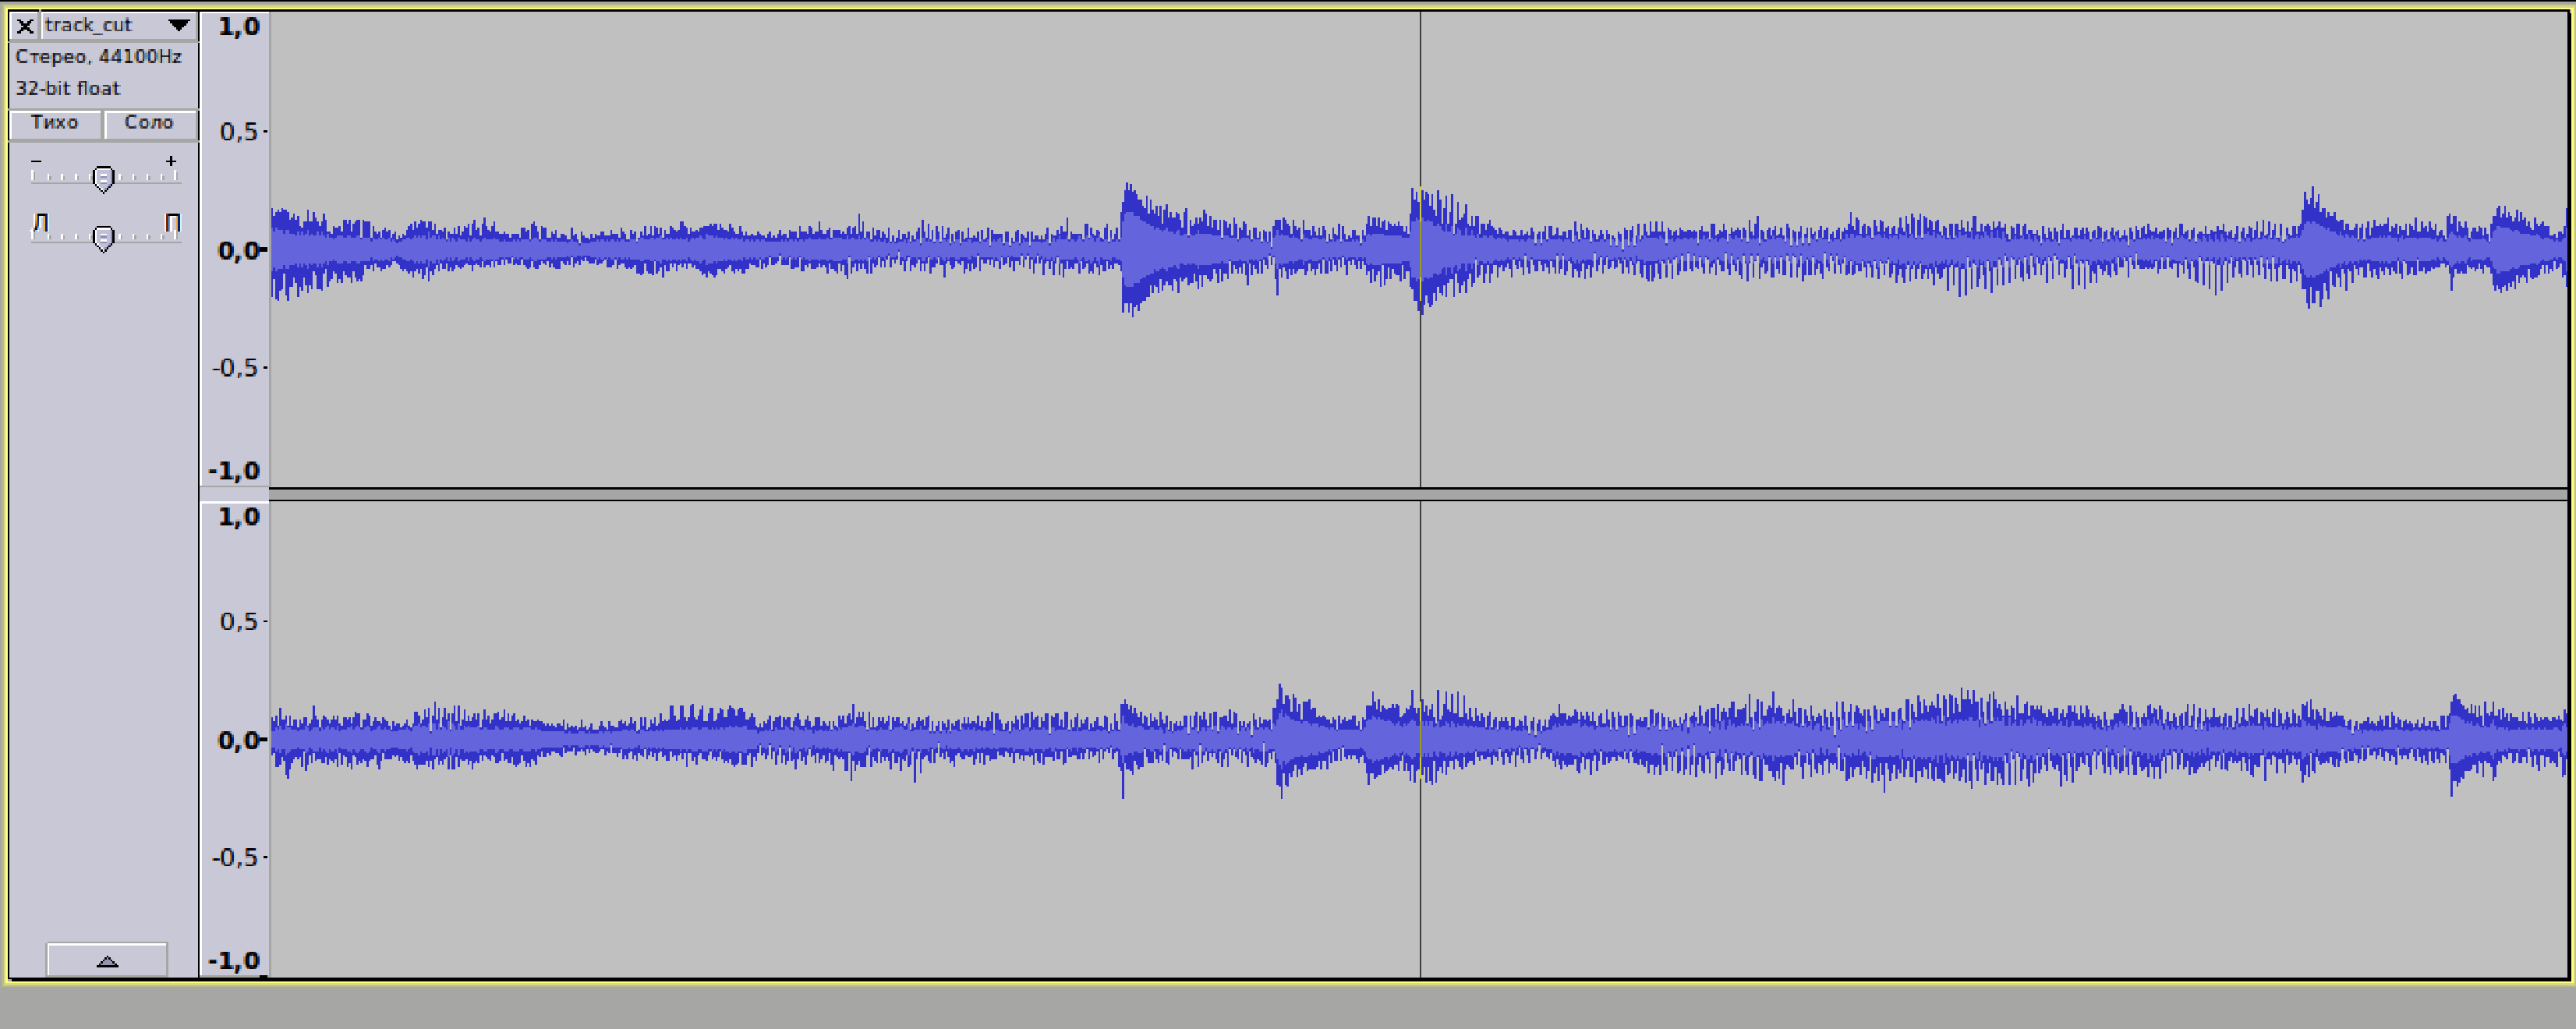
\includegraphics[scale=0.14]{attachments/sound_vawe.png}
	\caption{Изображение звуковой волны}
	\label{sec:analysus:sound_wave}
\end{figure}

Цифровой аудиосигнал представляет собой множество точек, которые расставлены на одинаковом расстоянии друг от друга. Расстояние между точками называется частотой дискретизации. Чем меньше интервал (выше частота дискретизации), тем шире частотный диапазон, который можно закодировать таким образом.

\begin{figure}[t]
\centering
	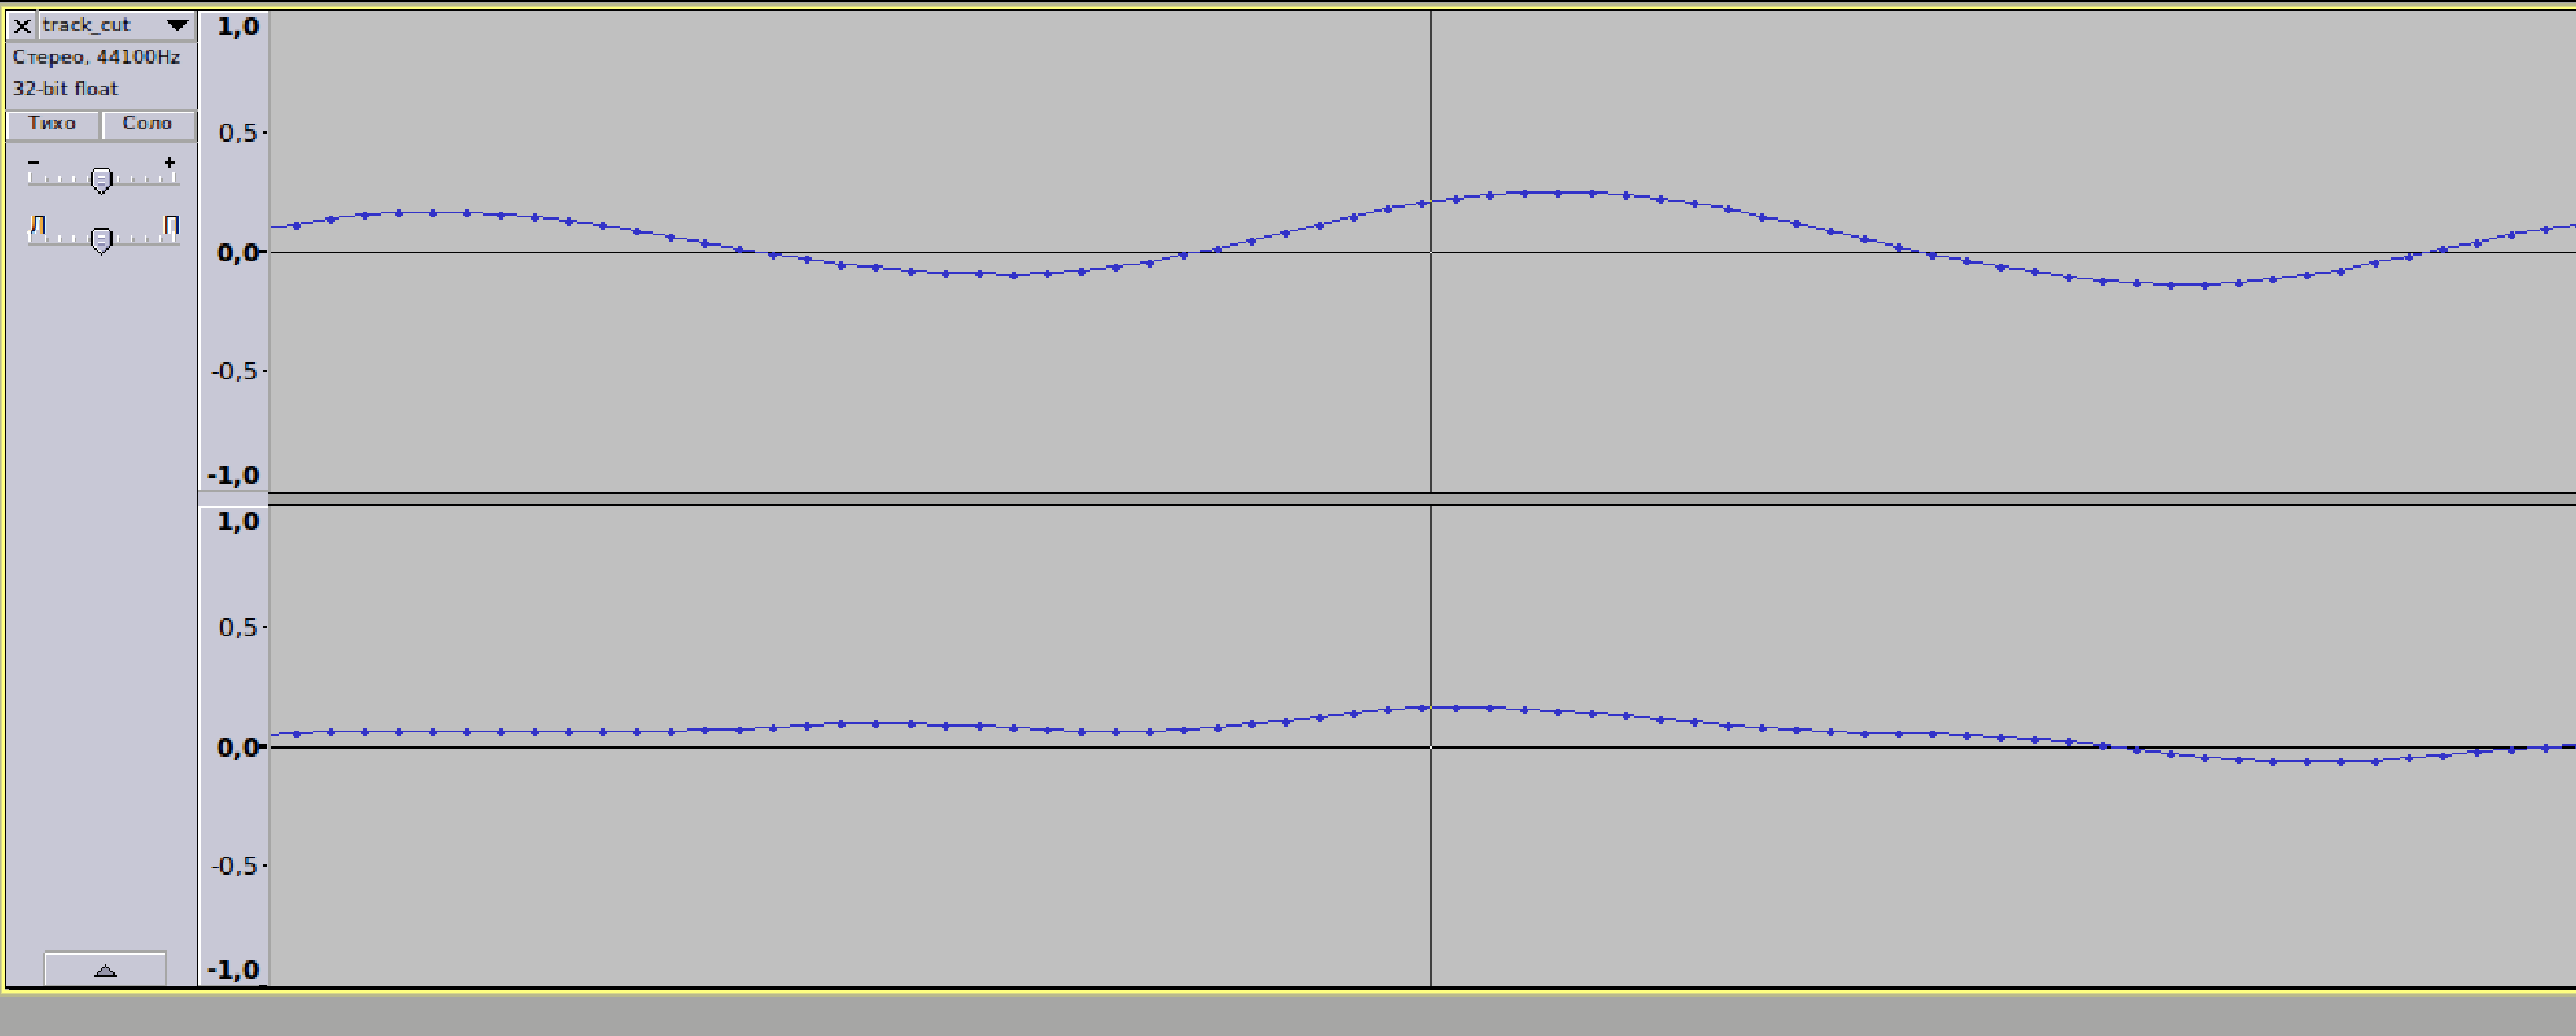
\includegraphics[scale=0.14]{sound_wave_hi.png}
	\caption{Изображение звуковой волны в большом разрешении}
	\label{sec:analysus:sound_wave_hi}
\end{figure}

Амплитуда колебаний зависит от времени звука и коррелирует с громкостью звука. А частота колебаний напрямую связана с высотой звука. Для того, чтобы получить информацию о частоте колебаний, необходимо применить преобразование Фурье. Преобразование Фурье позволяет разложить периодическую функцию в сумму гармонических с разными частотами. Коэффициенты гармонических функций при сложении будут давать нам те частоты, которые мы хотим получить.

При применении преобразования Фурье ко всей звуковой дорожке мы получим "смазанный" во времени спектр. Для того, чтобы получить спектр, не теряя временной составляющей, необходимо применить к сигналу оконное преобразование Фурье. Оконное преобразование Фурье отличается от обычного тем, что мы делим наш сигнал на короткие отрезки (окна) и применяем к каждому преобразование Фурье. По-сути мы получаем набор спектров - отдельно для каждого отрезка. В результате мы получим картинку, которой можно описать звуковую дорожку.

\begin{figure}[t]
\centering
	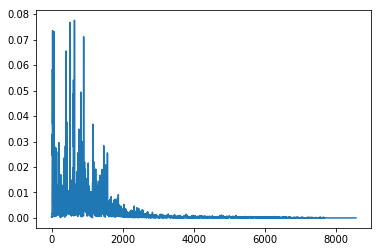
\includegraphics[scale=1]{spectrum.png}
	\caption{Спектральная характеристика}
	\label{sec:analysus:spectrum}
\end{figure}

Жанр композиции является высокоуровневой характеристикой. Для определения жанра необходимо разобраться, как человек воспринимает звук.

Ухо человека устроено так: звуковые волны смещают барабанную перепонку при взаимодействии с ней. Вибрации передаются во внутреннее ухо и считываются им. Смещение барабанной перепонки зависит от звукового давления, при том зависимость является не линейной, а логарифмической. Для измерения громкости принято использовать относительную шкалу - уровень звукового давления (измеряется в децибелах). Так же воспринимаемая громкость зависит и от частоты звука. Для оценки громкости звука используется логарифмическая единица измерения - фон. В шкале фонов, в отличие от децибелов, значения громкости связаны с чувствительностью на разных частотах человеческого уха. Частота 1000 Гц является чистым тоном, и уровень фона для неё численно равен уровню в децибелах. Для остальных частот используют поправки, которые представляют собой стандартизированное семейство кривых, называемых изофонами.

\begin{figure}[t]
\centering
	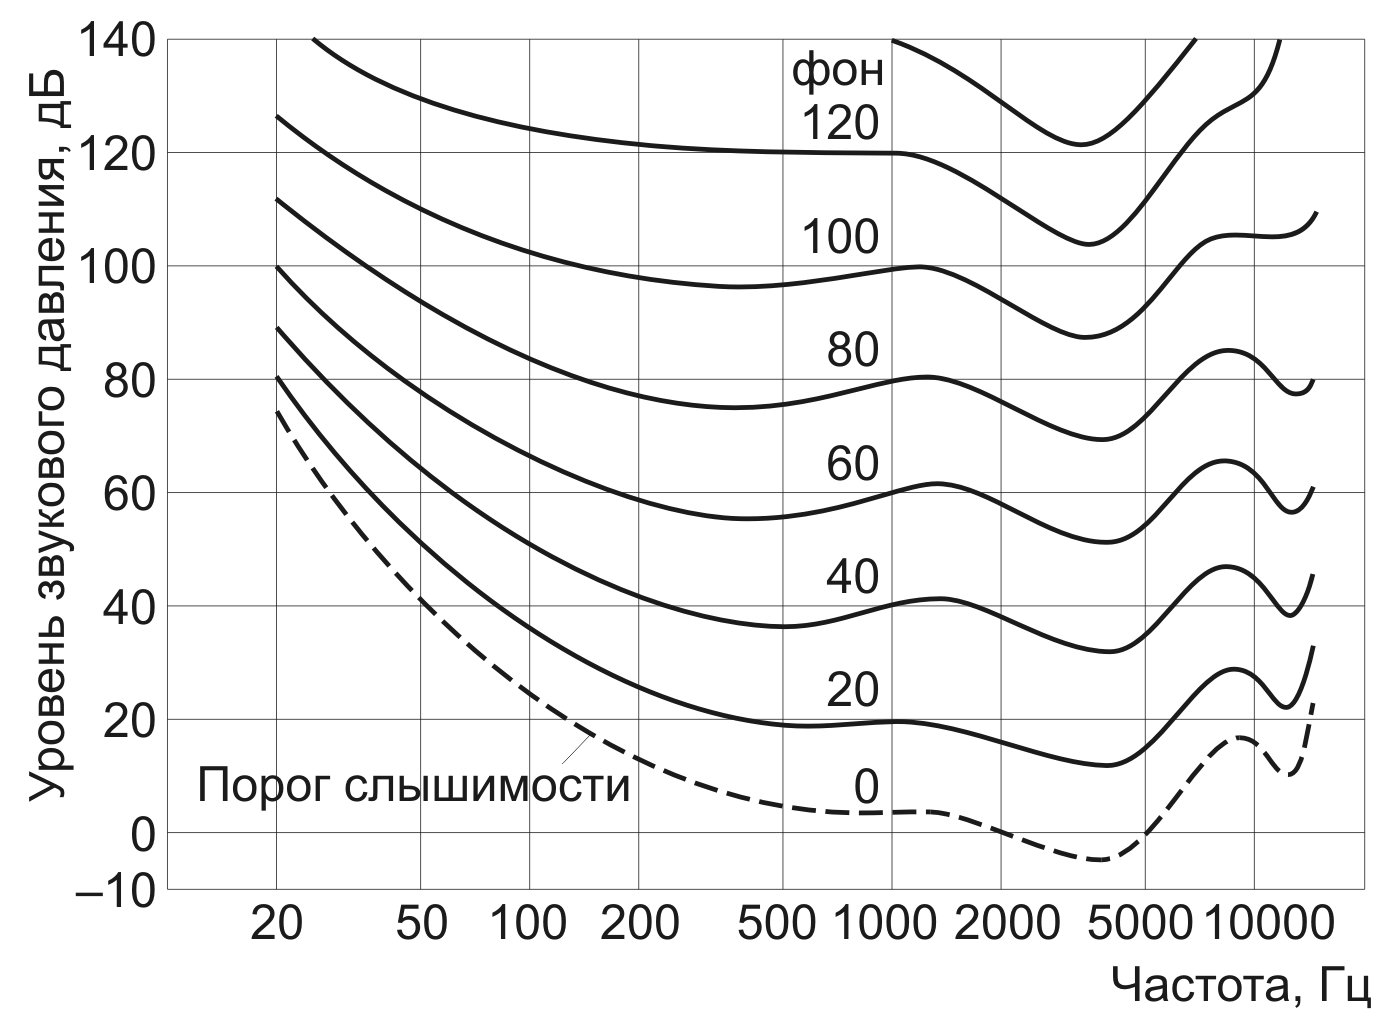
\includegraphics[scale=2]{Gromkost.png}
	\caption{Контур равных громкостей}
	\label{sec:analysus:sound_contur}
\end{figure}

Аналогично с громкостью, частота так же воспринимается человеческим ухом нелинейно. Для измерения воспринимаемой частоты человеческим ухом используется мел-шкала. Шкала основана на статистической обработке субъективного восприятия звука на больших данных. За 1000 мел взят звук с частотой 1000 Гц при уровне громкости 40 фон. За 0 мел взят звук частотой 20 Гц при уровне громкости 40 фон.

\begin{figure}[t]
\centering
	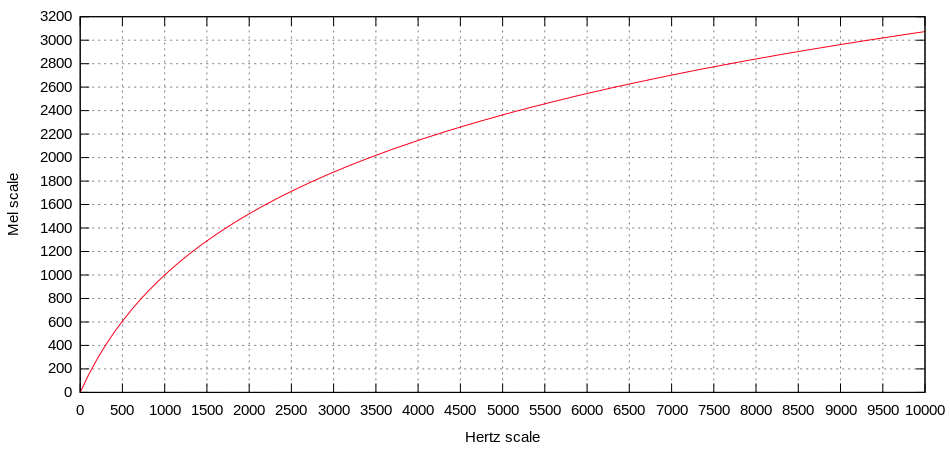
\includegraphics[scale=0.48]{mel-hz.png}
	\caption{Мел шкала}
	\label{sec:analysus:mel}
\end{figure}
